\chapter{Fitness Estimation}

This chapter explains a proposed strategy to calculate the fitness of
individuals in web-based IEC applications
using fuzzy logic. Before showing our strategy, it is necessary to explain how
the individual evaluation is made in the EvoDrawing application. Figure
\ref{fig:UI_ED} shows the user interface.
The main goal of this interaction is the evaluation of individuals, but
the first user action before starting to evaluate, is to login through the
Facebook \cite{facebook} social
platform account. The evaluation takes place through a
five star rating selection; this rate represents the degree of user
preference for an individual. The application keeps record of every user
activity by using the activity stream standard \cite{snell2014json}.
In these particular case activities represent the user's experience.

\begin{figure*}
\captionsetup{justification=centering,margin=2cm}
\centering
\setlength\fboxsep{0pt}
\setlength\fboxrule{0.7pt}
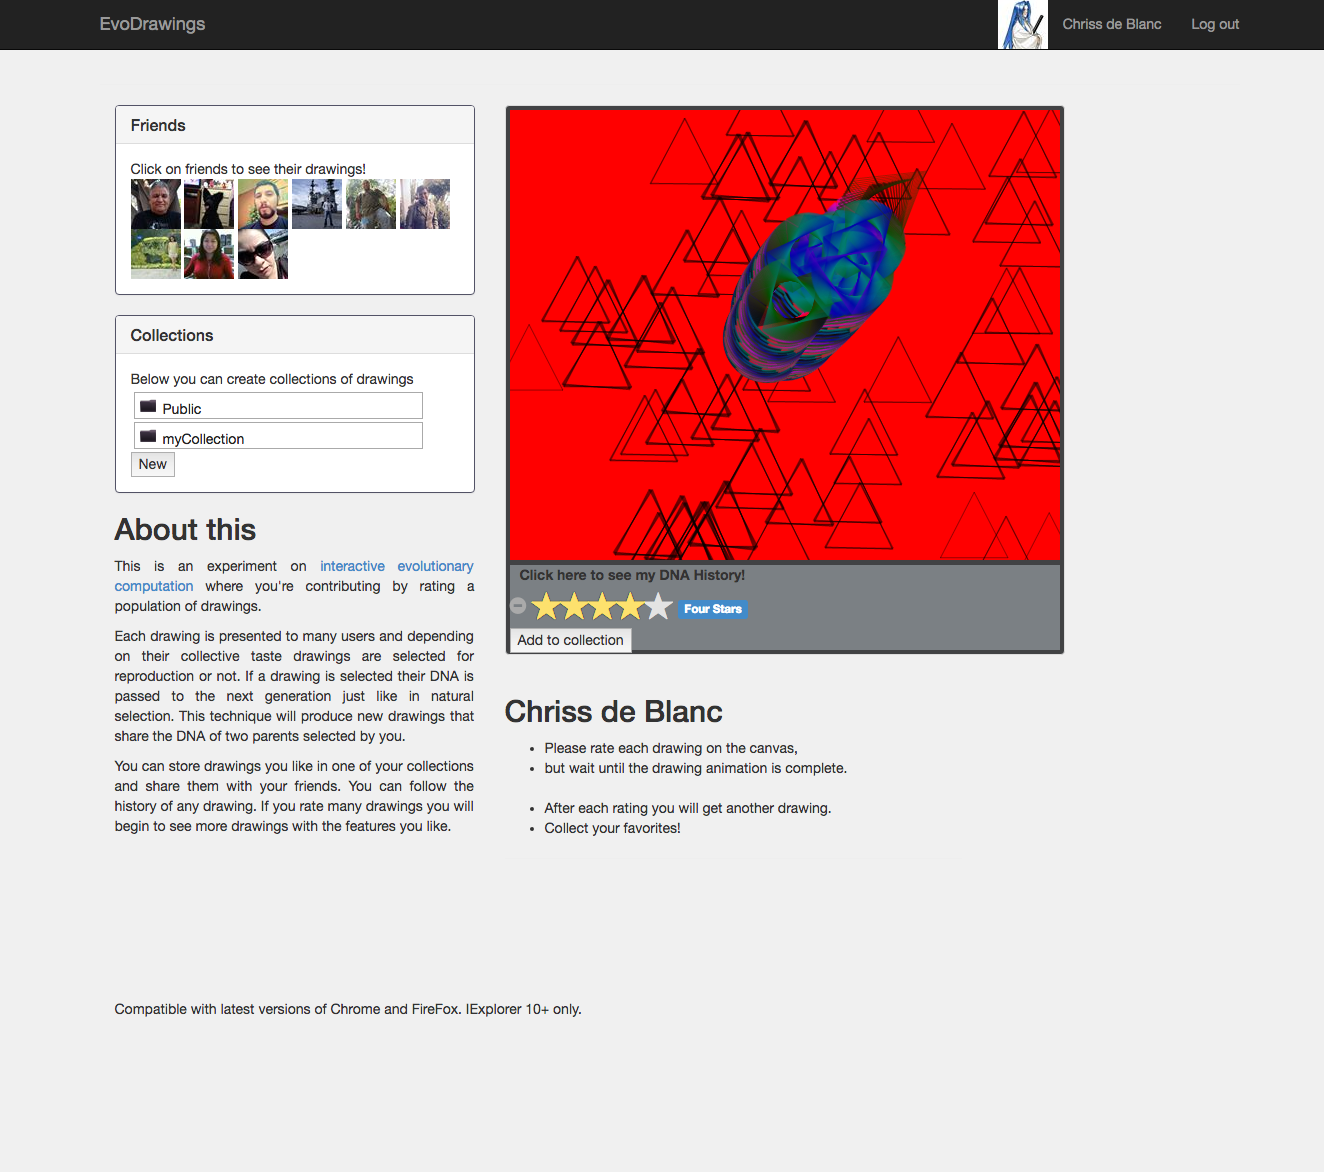
\includegraphics[width=12cm,height=10cm,keepaspectratio]{img/UI_ed01.png}
\caption{User interface ED01.}
\label{fig:UI_ED}
\end{figure*}

In this thesis the usage of fuzzy logic is proposed \cite{Zadeh1973} in order to
obtain the individual fitness trough a fitness function expression. It is used
by modeling a fuzzy Mamdani type inference system \cite{mamdani1975experiment}
\cite{mamdani1974application} that represents all the interaction of the
user-individual in given IEC application as Figure \ref{fig:fis01} shows. This
model was designed empirically. The model consists of two input variables, which
are the preference and the experience of the user as well as an output that we
called fuzzy rate. The first variable has three linguistic variables, which are
low, medium and high, representing the preferences of the users with triangular
membership functions over a range of 1 to 5. The second variable also has three
linguistic variables, which are low, medium and high representing the experience
with triangular membership functions over a range of 1 to 100. Finally we have
the output consisting of three consequent variables which are bad, normal and
good representing the fuzzy rate with triangular membership functions in a range
of 1-100.

\begin{figure*}
\captionsetup{justification=centering,margin=2cm}
\centering
\setlength\fboxsep{0pt}
\setlength\fboxrule{0.7pt}
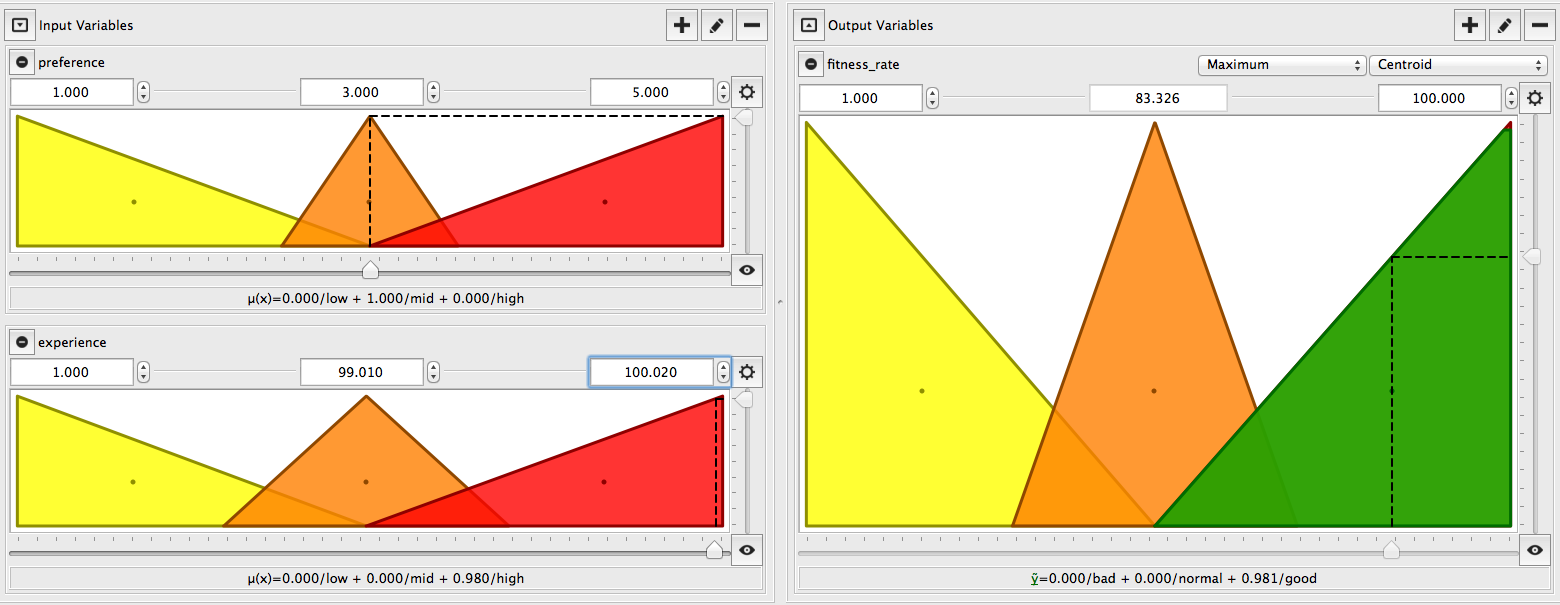
\includegraphics[width=12cm,height=10cm,keepaspectratio]{img/fuzzy_system_2_1.png}
\caption{Fuzzy System Mamdani Type.}
\label{fig:fis01}
\end{figure*}

Below we show the rules IF-THEN of the fuzzy system:

\begin{enumerate}
	\item \textit{If \textbf{preference} is low and
		\textbf{experience} is low then \textbf{fuzzy\_rate} is bad.}
	\item \textit{If \textbf{preference} is mid and
		\textbf{experience} is low then \textbf{fuzzy\_rate} is bad.}
	\item \textit{If \textbf{preference} is high and
		\textbf{experience} is low then \textbf{fuzzy\_rate} is normal.}
	\item \textit{If \textbf{preference} is low and
		\textbf{experience} is mid then \textbf{fuzzy\_rate} is bad.}
	\item \textit{If \textbf{preference} is mid and
		\textbf{experience} is mid then \textbf{fuzzy\_rate} is normal.}
	\item \textit{If \textbf{preference} is high and
		\textbf{experience} is mid then \textbf{fuzzy\_rate} is good.}
	\item \textit{If \textbf{preference} is low and
		\textbf{experience} is high then \textbf{fuzzy\_rate} is normal.}
	\item \textit{If \textbf{preference} is mid and
		\textbf{experience} is high then \textbf{fuzzy\_rate} is good.}
	\item \textit{If \textbf{preference} is high and
		\textbf{experience} is high then \textbf{fuzzy\_rate} is good.}

\end{enumerate}

These rules will give us a fuzzy rate value as a result of the interaction with
the users in given IEC application, this value needs to be defuzzified by the
centroid method in order to be used in our fitness expression, given by the
equation\ref{eq:fitfunc_02}. This expression is responsible of representing the
individual fitness.

\begin{equation}\label{eq:fitfunc_02}
\displaystyle fitness=\frac{\sum_{i=0}^{n}x_{i}+f(y_{i})}{\sum_{i=0}^{n}f(y_{i})}
\end{equation}

Where $n$ represents the number of users that have evaluated the
individual, $x$ is the rate of preference for the individual given by the user,
$y$ is a function that calls the fuzzy system in order to have the fuzzy rate.
This function has as a parameter the rate $x$ and the user experience level.
The user experience level
is given by the total activities that user has at the moment. In each
activity we assign the score, for example if the user log in (join) to the
application we assign 5 points, if the user evaluates (likes) an individual we
give 3 points, etc; in Figure \ref{fig:fitnessFlow} shows the flow for assigning fitness to
the individual.

\begin{figure*}
\captionsetup{justification=centering,margin=2cm}
\centering
\setlength\fboxsep{0pt}
\setlength\fboxrule{0.7pt}
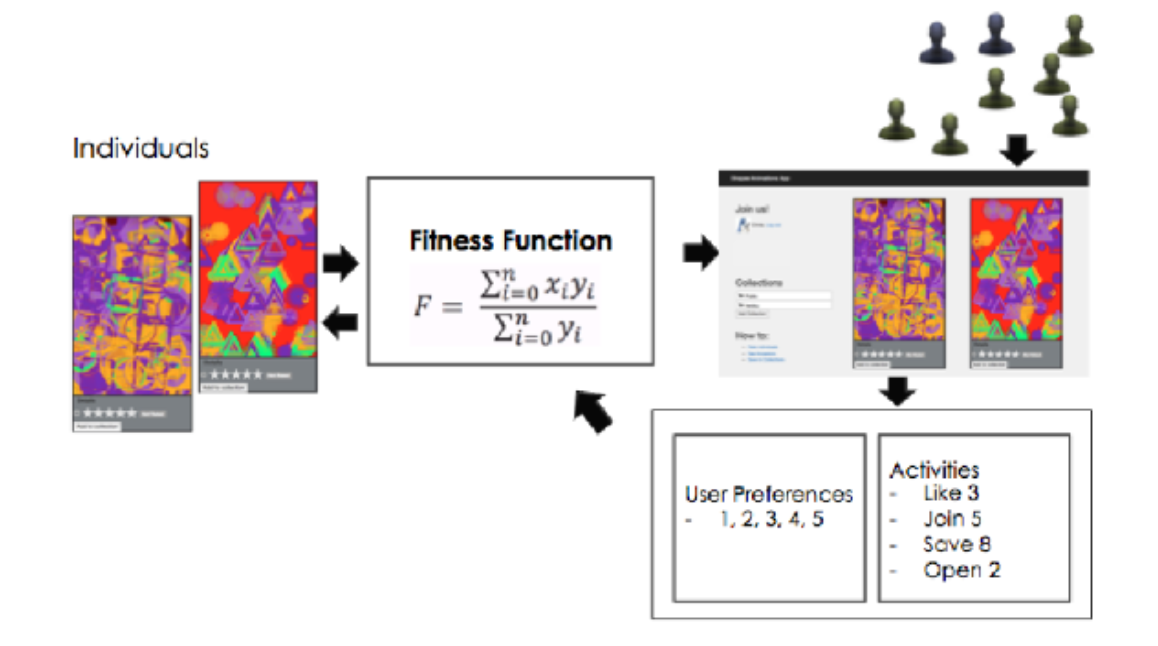
\includegraphics[width=12cm,height=10cm,keepaspectratio]{img/fitnessFlow.png}
\caption{Fitness Flow.}
\label{fig:fitnessFlow}
\end{figure*}



Where $n$ represents the number of users that have evaluated the
individual, $x$ is the rate of preference for the individual given by the user,
$y$ is a function that calls the fuzzy system in order to have the fuzzy rate.
This function has as a parameter the rate $x$ and the user experience level.
The user experience level
is given by the total activities that user has at the moment. In each
activity we assign the score, for example if the user log in (join) to the
application we assign 5 points, if the user evaluates (likes) an individual we
give 3 points, etc; in Figure \ref{fig:fitnessFlow} shows the flow for assigning fitness to
the individual.
